\chapter{Visor web dinámico de objetos 3D}\label{cap.visor3d}
En este capítulo se trata la creación de un nuevo visor de primitivas 3D (objetos, puntos y segmentos) con tecnologías web. Este visor, al que se ha nombrado como 3DVizWeb\footnote{\url{https://github.com/RoboticsURJC-students/2017-tfg-roberto-perez/tree/master/3DVizWeb}}, abre la posibilidad de obtener datos 3D por una o varias cámaras o sensores y mostrar una representación 3D de los mismos.
\section{Diseño}
Este visor está elaborado usando JavaScript y HTML5 como lenguajes de programación, y se usa el \textit{middleware} ICE para la interconexión con los clientes que envían los datos a mostrar. En la figura 5.1 se muestra su diagrama de bloques:

\begin{figure}[H]
  \begin{center}
    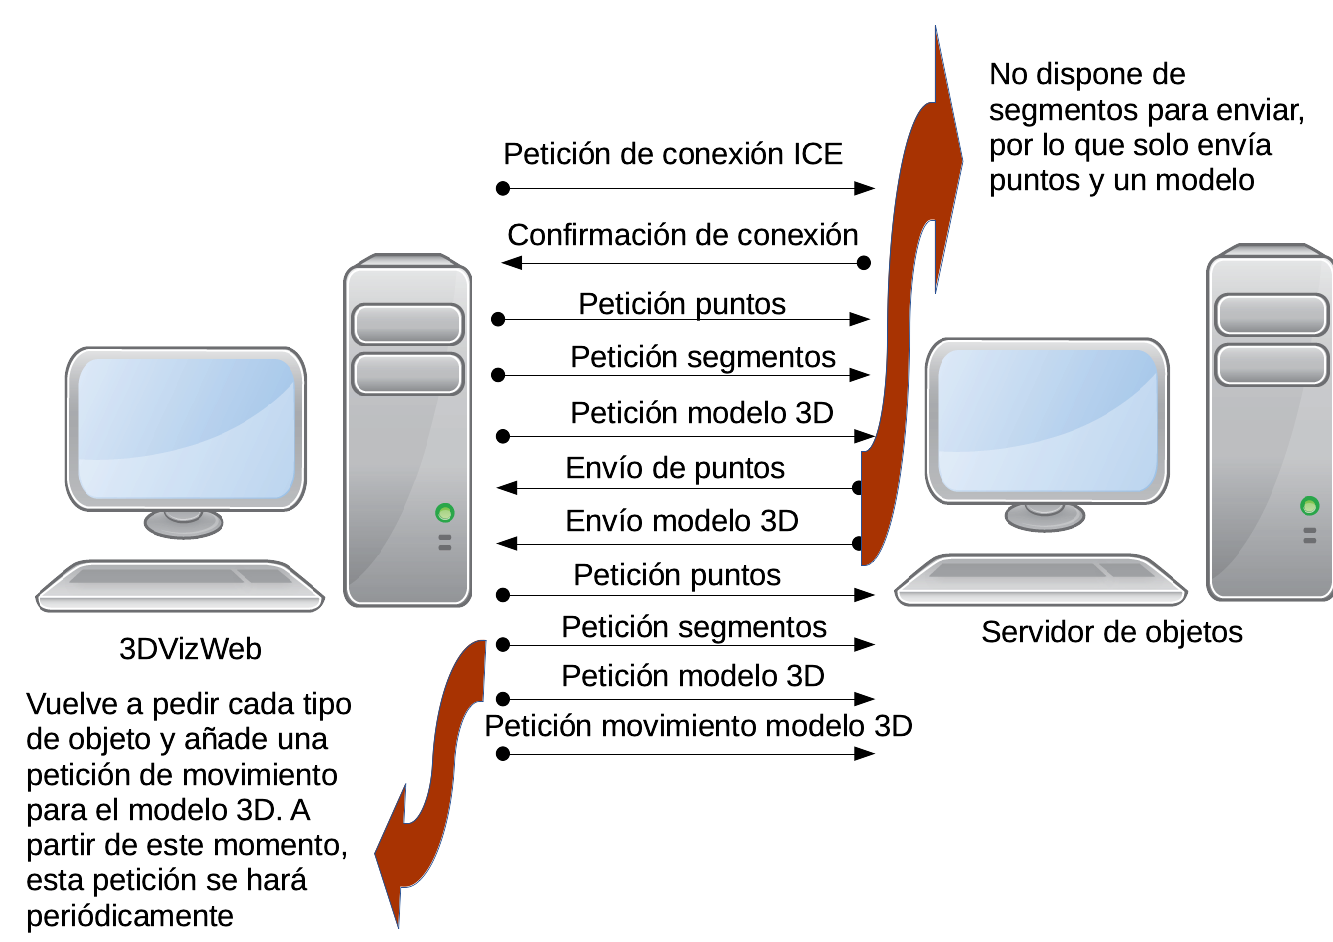
\includegraphics[width=0.8\textwidth]{figures/esquemavisor.png}
		\caption{Ejecución típica del visor 3D}
		\label{fig.diseno3dviz}
		\end{center}
\end{figure}

En la figura 5.2 se muestra el diseño del visor de una manera más detallada:

\begin{figure}[H]
  \begin{center}
    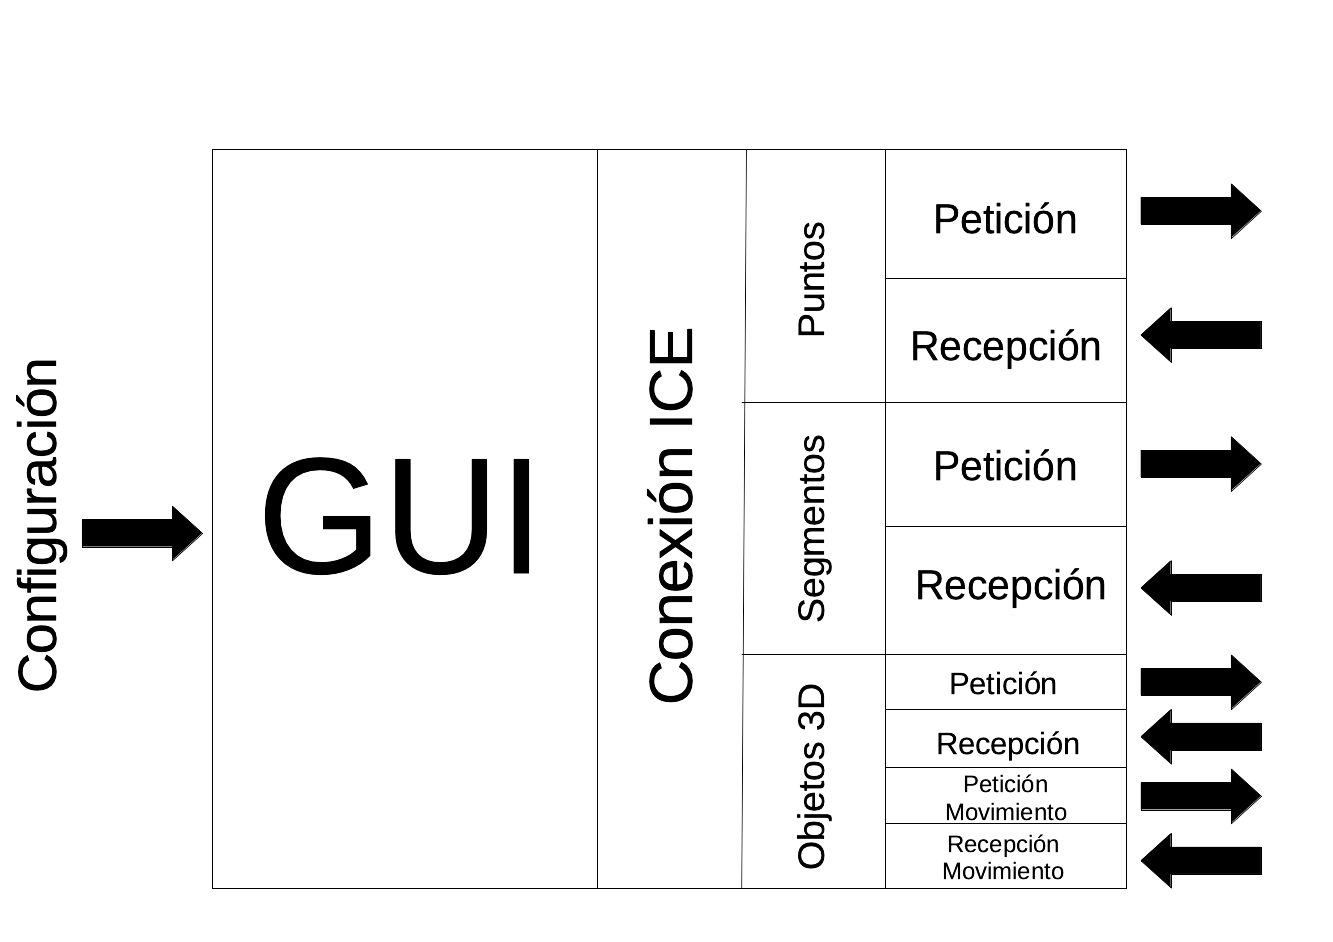
\includegraphics[width=0.8\textwidth]{figures/diseno3dviz.png}
		\caption{Diagrama de bloques del visor 3D}
		\label{fig.diseno3dviz}
		\end{center}
\end{figure}
La herramienta está dividida en dos partes: la interfaz gráfica y las conexiones ICE.

La parte correspondiente a la interfaz gráfica es la que da origen al visor y marca cómo se definen cada uno de los tipos de objetos que es capaz de mostrar. Hay tres tipos de primitivas 3D que el visor es capaz de visualizar: puntos, segmentos y objetos.

Las conexiones ICE con el servidor incluyen varias partes claramente diferenciadas. Estas partes corresponden a la petición y recepción de cada tipo de primitiva al servidor, haciendo especial hincapié en los objetos 3D que contarán con las peticiones y recepciones propias para mostrar nuevos objetos. El visor admite los formatos de archivo del tipo ``dae'' y del tipo``obj''. Estos dos formatos son los más utilizados a la hora de crear objetos 3D y por tanto se considera que dando soporte a estos se permite usar cualquier objeto que se desee. Los objetos se podrán mover en 3D y el visor ofrece mecanismos eficientes para que las aplicaciones, mediante  peticiones y recepciones, puedan mover los objetos existentes en la escena que se está visualizando.

\section{Configuración}
Dado que el visor en su interfaz gráfica únicamente muestra la escena donde se visualizan los objetos, es necesario utilizar una alternativa para configurar los datos de conexión (ip y puerto de escucha) y otros parámetros configurables (posición inicial de la cámara, tamaño de los puntos, tamaño de los segmentos y periodo de tiempo entre peticiones de cada tipo de objeto) antes de arrancar el visor. Para realizar está configuración se vuelve a utilizar un archivo en formato YAML, como se explica en la sección 4.1.6 de este trabajo.

Los parámetros que se pueden configurar para el visor son los siguientes:
\begin{itemize}
\item Dirección IP. Por defecto es ``localhost''
\item Puerto. Por defecto es ``11000''
\item Tiempo de refresco para la petición de puntos en milisegundos. Por defecto son 1000 ms
\item Tiempo de refresco para la petición de segmentos en milisegundos. Por defecto son 1000 ms
\item Tiempo de refresco para la petición de objetos 3D en milisegundos. Por defecto es 1 ms
\item Tiempo de refresco para la petición del movimiento de objetos en milisegundos. Por defecto son 1000 ms
\item Grosor de los segmentos en píxeles. Por defecto son 2 píxeles.
\item Tamaño de los puntos en píxeles. Por defecto son 8 píxeles.
\item Posición inicial de la cámara desde que se observa la escena. Está formada por las coordenadas ``x'', ``y'' y ``z'' , siendo por defecto 50, 20 y 100 respectivamente.
\end{itemize}

\section{Interfaz gráfica}
La interfaz gráfica del visor está diseñada usando WebGL, y más concretamente usando la biblioteca \texttt{Three.js} descrita en capítulos anteriores. La interfaz gráfica de la aplicación, la ventana, la ocupa íntegramente el visor 3D, no tendrá ningún elemento adicional como pueden ser botones o diales. La escena 3D muestra inicialmente una rejilla que hará de plano horizontal, cuyo centro será la posición (0, 0, 0) del eje de coordenadas. Además ha sido necesario añadir iluminación y una cámara para visualizar la escena desde ella.

\subsection{Escena base}
El visor está contenido dentro de un elemento HTML \texttt{<canvas>}. En este elemento se crea una nueva escena usando la función de \texttt{Three.js} \texttt{THREE.Scene()} y se renderiza usando \texttt{THREE.WebGLRenderer()}. Posteriormente se crea una cámara con perspectiva utilizando \texttt{THREE.PerspectiveCamera()} ubicándola en una posición predeterminada (la indica en el archivo de configuración) y podrá ser controlada mediante teclado o ratón. Finalmente, para visualizar correctamente la escena se añaden varias luces puntuales a lo largo de la misma, así como una iluminación de ambiente utilizando \texttt{THREE.PointLight()} y \texttt{THREE.AmbientLight()} pasándole como parámetros el color de la luz y la intensidad de la misma.

Una vez tenemos una escena completamente visible, se procede a crear y añadir la rejilla. La función existente en la biblioteca \texttt{Three.js} \texttt{new THREE.GridHelper()} permite definirla muy fácilmente introduciendo por parámetro a la función la separación, cantidad y color de las líneas de división que generan la rejilla. Para añadirla a la escena, basta con usar \texttt{.add(rejilla)}. Estos elementos forman la escena base del visor.

\begin{figure}[H]
  \begin{center}
    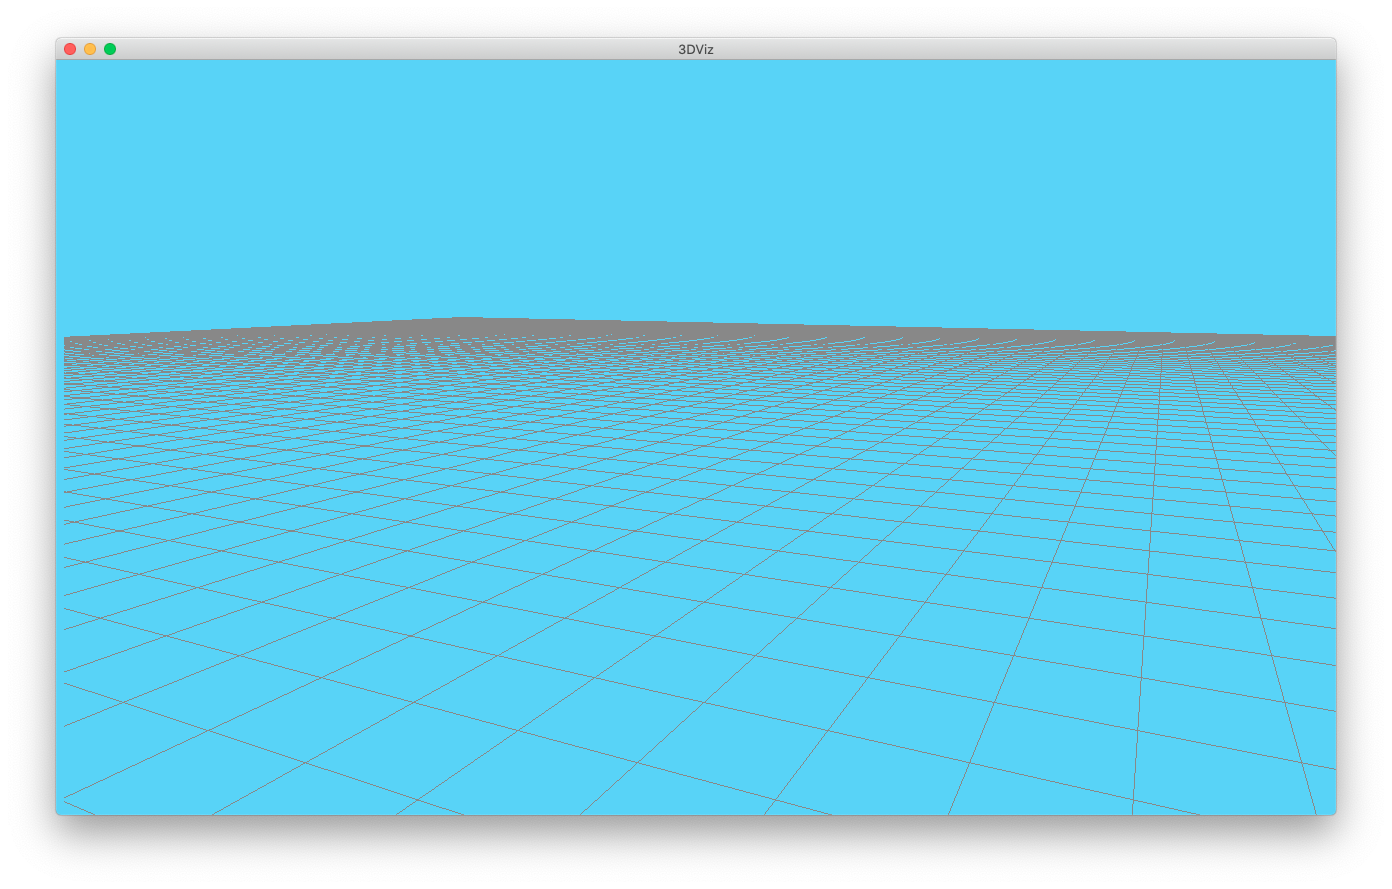
\includegraphics[width=0.8\textwidth]{figures/interfazinicial.png}
		\caption{Interfaz gráfica con la escena base del visor}
		\label{fig.interfazinicial}
		\end{center}
\end{figure}

\subsection{Visualización de puntos}
Un punto es el elemento geométrico más simple que es posible representar. Pese a ello proporciona al visor la capacidad de realizar representaciones complejas mediante el uso de una gran cantidad de puntos. Para representar puntos, únicamente es necesario una posición en el eje de coordenadas, el tamaño del punto y el material o color que se quiera darle. 
La biblioteca \texttt{Three.js} proporciona una serie de elementos para facilitar la creación de puntos. El código se muestra en el cuadro 5.2.


\begin{lstlisting}[caption= Creación y visualización de puntos, label=cod.crearpunto]
function addPoint (point){
	var geometry = new THREE.Geometry();
	geometry.vertices.push( new THREE.Vector3(point.x,point.z,point.y));
	var material = new THREE.PointsMaterial( { size: 8, sizeAttenuation: false, 
										alphaTest: 0.5, transparent: true } );
	material.color.setRGB( point.r, point.g, point.b);
	var particles = new THREE.Points( geometry, material );
	particles.name ="points";
	scene.add( particles );}
\end{lstlisting}

Primero es necesario indicar que se está creando una figura geométrica para posteriormente definirla. Al tratarse de un punto, solo va a tener un vértice por lo que al definir la geometría se indica que serán vertices pero únicamente se proporciona uno de ellos mediante un vector ``x'', ``y'' y  ``z'', que serán las coordenadas centrales del punto a representar. Dado que el sistema de coordenadas de obtención en WebGL de los datos no se corresponde con el sistema de coordenadas gráficas de la escena, hay que realizar una conversión. Si recibimos un punto con coordenadas (x,y,z), en la escena corresponderán a (x,z,y). 


Una vez definida la geometría lo siguiente es definir el tamaño del punto, su aspecto y su color. El tamaño indicado en el código es de 8 píxeles, sin embargo este tamaño es configurable a través del fichero de configuración. El color del punto se define mediante sus componentes RGB, que vienen indicadas por el servidor que transmite el punto. Las componentes vendrán separadas en ``R'', ``G'' y ``B'', y su valor oscilará entre ``0'' y ``1'' (se corresponde con el valor ``255'') para cada una de ellas.

Finalmente creamos el punto a partir de la geometría y el material proporcionado, le atribuimos el nombre ``punto'' para poder borrarlo discrecionalmente si así se desea, y se añade a la escena.
Esta función será invocada cada vez que se reciba uno o más puntos procedentes del servidor. La figura 5.4 muestra varios puntos coloreados en el visor.
\begin{figure}[H]
  \begin{center}
    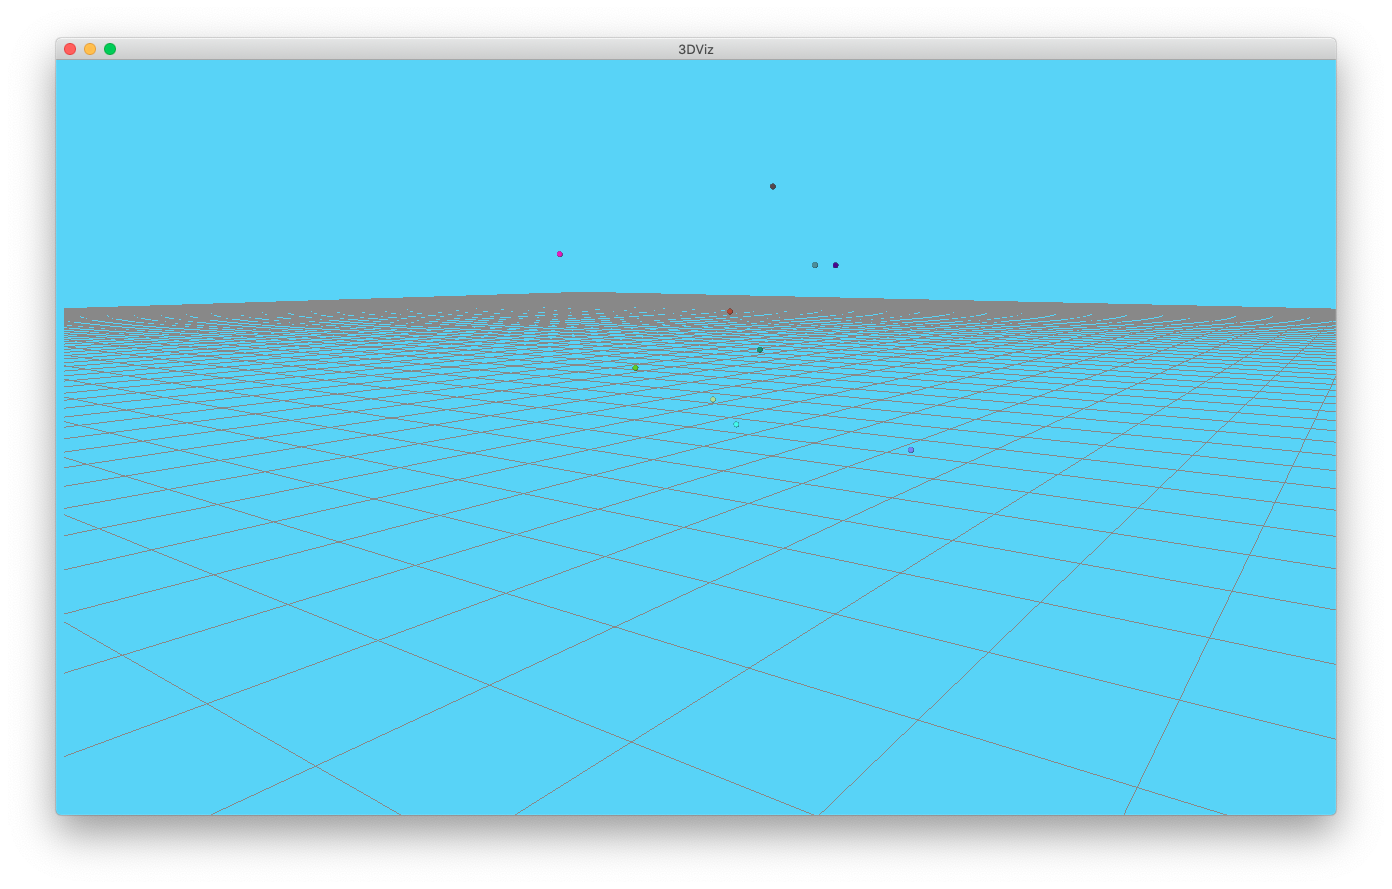
\includegraphics[width=0.8\textwidth]{figures/visualizarpuntos.png}
		\caption{Varios puntos de distintos colores visualizados en el visor}
		\label{fig.visualizarpuntos}
		\end{center}
\end{figure}
\subsection{Visualización de segmentos}
El segmento es otro de los elementos fundamentales de la geometría y se puede definir cómo un fragmento de recta que está comprendido entre dos puntos. Teniendo en cuenta esto, para  representarlo únicamente es necesario las coordenadas de dos puntos, el grosor del segmento y el color del mismo. En el cuadro 5.3 se muestra el código para la creación de un segmento.


\begin{lstlisting}[caption= Creación y visualización de segmentos, label=cod.crearsegmento]
function addLine(segment){
	var geometry = new THREE.Geometry();
	geometry.vertices.push(
		new THREE.Vector3(segment.fromPoint.x, segment.fromPoint.z, 
							segment.fromPoint.y),
		new THREE.Vector3(segment.toPoint.x, segment.toPoint.z, 
							segment.toPoint.y));
	var material = new THREE.LineBasicMaterial();
	material.color.setRGB(segment.r, segment.g, segment.b);
	material.linewidth = 2;
	line = new THREE.Line(geometry,material);
	line.name = "line";
	scene.add(line);}
\end{lstlisting}

La estructura es muy similar que la función para crear un punto y al igual que allí, se necesita definir la geometría. En este caso vamos a tener dos vértices en lugar de uno (dos puntos). El primero es desde el lugar donde comience el segmento, y el segundo el lugar donde termina. En otras palabras, el segmento será la unión entre el primer vértice con el segundo. Las coordenadas de estos dos puntos serán proporcionadas por el servidor. Al igual que en el caso del punto, el sistema de coordenadas del servidor no coincide con el sistema del visor, por lo que se debe realizar la misma conversión, es decir la coordenada ``z'' que envíe el servidor, se corresponde a la coordenada ``y'' del visor, y viceversa.

Posteriormente se definen el material y aspecto del segmento proporcionando el grosor y el color. En el código anterior, el grosor es de 2 píxeles, sin embargo este parámetro es configurable mediante el fichero de configuración. El color, por el contrario, viene definido por la aplicación mediante sus componentes RGB, que al igual que para el caso del punto, vienen repartidas en ``R'', ``G'' y ``B'', valiendo entre ``0''  y ``1'' (corresponde al valor ``255'').

Finalmente se crea el segmento a partir de la geometría y el material proporcionado, dándole el nombre ``line'' para poder borrar selectivamente solo los segmentos. Una vez generado el elemento, se añade a la escena. Esta función será la invocada cada vez que se reciba uno o más segmentos. La figura 5.5 muestra varios segmentos en el visor.

\begin{figure}[H]
  \begin{center}
    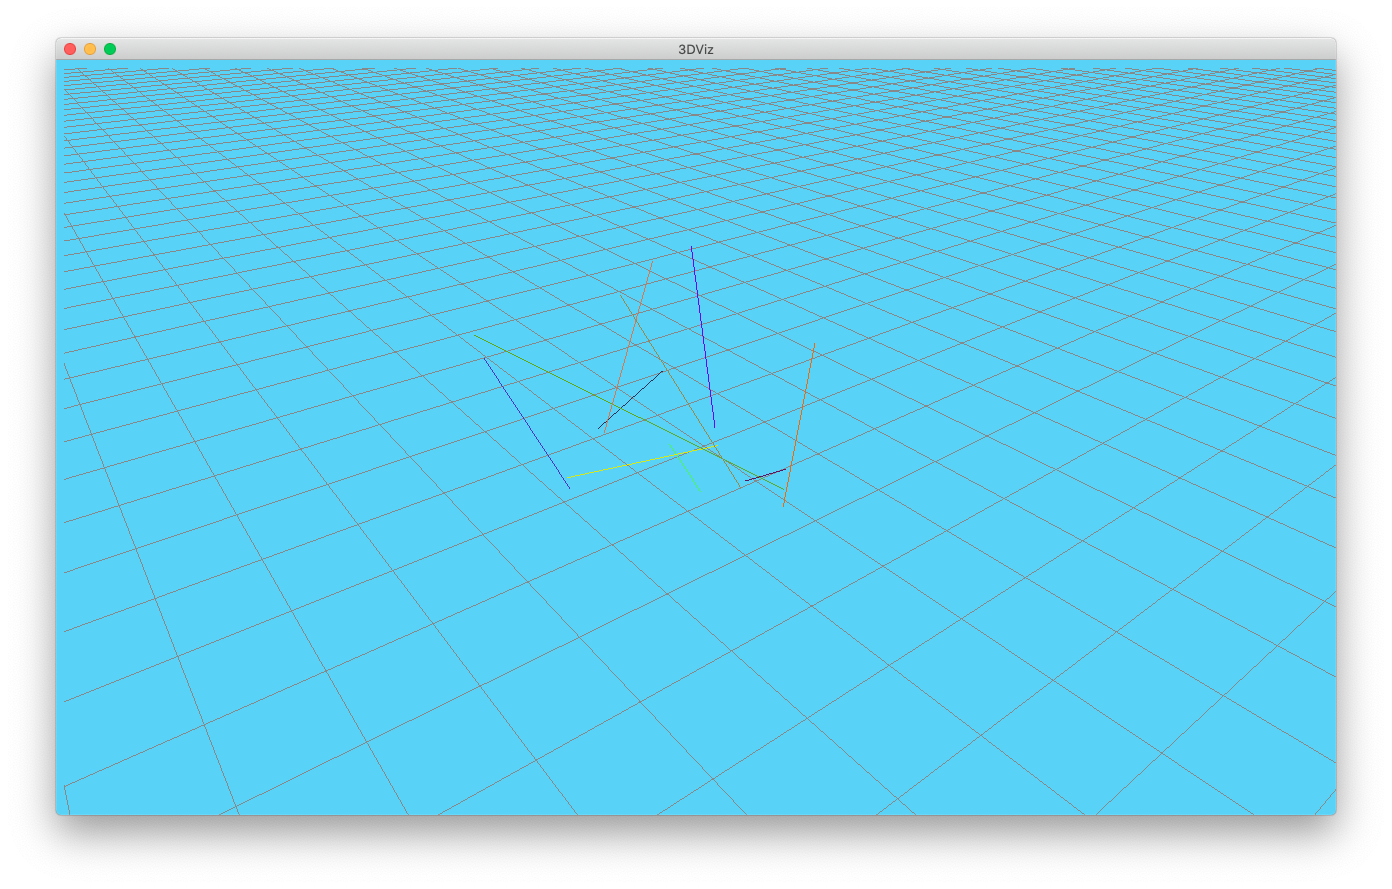
\includegraphics[width=0.8\textwidth]{figures/visualizarlineas.png}
		\caption{Varios segmentos de distintos colores visualizados en el visor}
		\label{fig.visualizarsegmentos}
		\end{center}
\end{figure}

\subsection{Visualización de objetos 3D}
Un objeto 3D es una representación matemática de un objeto tridimensional cuya geometría se puede guardar en un archivo. El visor es capaz de representar dos formatos diferentes de estos archivos, ``obj'' y ``dae'', y moverlos cuando la aplicación lo requiera. 

\subsubsection{Creación y visualización de los objetos 3D}
Los objetos 3D pueden ser recibidos bien a través del archivo completo como texto plano, o bien a través de una URL. El visor será capaz de representar el objeto 3D y ubicarlo en la posición indicada. El código del cuadro 5.4 muestra cómo identificar si el objeto viene como texto plano o URL, para invocar a la función correspondiente dependiendo el formato del objeto.


\begin{lstlisting}[caption= Creación y visualización de objetos 3D, label=cod.crearobjetos3d]
function addObj(obj,pos){
	var type = obj.obj.split(":");
	if (type[0] == "https" || type[0] == "http") {
		var url = obj.obj
	} else{
		var file = new Blob([obj.obj], {type:'text/plain'});
		var url  = window.URL.createObjectURL(file);
	}
	if (obj.format == "obj"){
		loadObj(url, obj,pos)
	} else if (obj.format == "dae") {
		loadDae(url,obj.pos);
	}
}
\end{lstlisting}
Cuando se recibe el objeto procedente de la plicación, lo primero que se hace es trocear el mensaje para analizarlo y esclarecer si lo que se está enviando es el archivo completo o una URL al archivo. De tratarse de una URL, debe contener ``https://'' o ``http://'', se puede trocear mediante ``:'' y, con una sentencia condicional verificar si la primera parte de la separación es ``https'', ``http'' u otra cosa. En caso de no ser ``https'' o ``http'', lo que lo que se ha recibido es el objeto completo y se debe generar un archivo virtual utilizando el objeto \textit{Blob} (objeto que representa un fichero) y posteriormente generar una URL virtual, ya que se ha recibido como texto plano y para visualizarlo es necesario que el objeto tenga una URL local al mismo. 

Una vez se tiene la URL del objeto, es necesario saber el formato del archivo del objeto (``obj'' o ``dae''), ya que no se carga el objeto de la misma forma. Identificar el formato es sencillo, ya que vendrá indicado por la aplicación y, dependiendo del formato, se invoca a la función de procesamiento correspondiente pasando por parámetro la URL y la posición deseada del objeto en el visor (coordenadas y orientación del objeto) recibidas del servidor.

\begin{itemize}
\item {\textbf{\underline{Representación de objetos del tipo obj}}

Un archivo con formato ``obj'' es conocido como Wavefront 3D Object File y el formato fue desarrollado por Wavefront Technologies. Es usado para un objeto tridimensional que contiene las coordenadas 3D (líneas poligonales y puntos), mapas de textura, y otra información de objetos. La biblioteca Three.js proporciona un API para cargar y mostrar un objeto de este tipo a través de una URL. 

El código del cuadro 5.5 carga y muestra un objeto ``obj'':


\begin{lstlisting}[caption= Carga y visualización de objetos ``obj'', label=cod.objetosobj]
function loadObj(url,obj,pose3d){
	var loader = new THREE.OBJLoader();
	loader.load(
		url,
		function(object){
			object.name = obj.id;
			id_list.push(obj.id);
			object.position.set(pose3d.x, pose3d.z, pose3d.y);
			object.rotation.set(pose3d.rx*toDegrees, pose3d.rz * toDegrees, 
							pose3d.ry * toDegrees);
			scene.add(object);
		},
		function (xhr){
		},
		function (error){
			console.log(error);
		});
}
\end{lstlisting}

Lo primero que hace es inicializar el API de Three.js para cargar un objeto ``obj'' y llama a la función del API encargada de cargar el objeto. Esta función tiene como parámetros la URL y otras tres funciones más. La primera es la encargada de cargar el objeto y mostrar el mismo en el visor, la segunda se ejecuta mientras se está cargando el objeto (por ejemplo, para mostrar una barra de progreso) y la última se ejecutará si ocurre algún error durante la carga. La primera función es la importante, en ella identificamos al objeto dándole un \texttt{id} previamente establecido y lo añadimos a un \texttt{array} para poder borrarlo o moverlo posteriormente. También posiciona el objeto en 3D mediante las coordenadas enviadas por la aplicación. Igualmente orienta el objeto 3D mediante la rotación correspondiente a cada eje, que es enviada en radianes y se debe convertir a grados.
Finalmente, se añade el objeto al visor.}

\item{\textbf{\underline{Representación de objetos del tipo dae}}

El formato ``dae'' de ficheros, también conocido como ``Collada'', es un formato de archivos 3D utilizado para el intercambio activo entre programas de gráficos y basado en el esquema XML Collada. La biblioteca Three.js proporciona un API para la carga y visualización de este formato a partir de una URL. El código del cuadro 5.6 carga y muestra un objeto ``dae'':

\begin{lstlisting}[caption= Carga y visualización de objetos ``dae'', label=cod.objetosdae]
function loadDae (url,obj,pose3d){
	var loader = new THREE.ColladaLoader();
	loader.load(url, 
		function (object) {
			object = object.scene;
			object.name = obj.id;
			id_list.push(obj.id);
			object.position.set(pose3d.x, pose3d.z, pose3d.y);
			object.rotation.set(pose3d.rx, pose3d.rz, pose3d.ry);
			scene.add( object );		
		},
		function (xhr){
		},
		function (error){
			console.log(error);
		});
}
\end{lstlisting}
Como se puede apreciar, el código es igual que el utilizado para el formato ``obj'', únicamente cambian la inicialización del API que en este caso es el API para cargar un archivo ``dae'' y la obtención del objeto, ya que se debe referenciar al mismo para poder cargarlo en el visor. El resto del código es el mismo para ambos casos.}
\end{itemize}
Estas funciones de carga serán invocadas cada vez que se reciba un objeto nuevo que mostrar. La figura 5.6 muestra dos objetos (cada uno de un formato) en el visor.

\begin{figure}[H]
  \begin{center}
    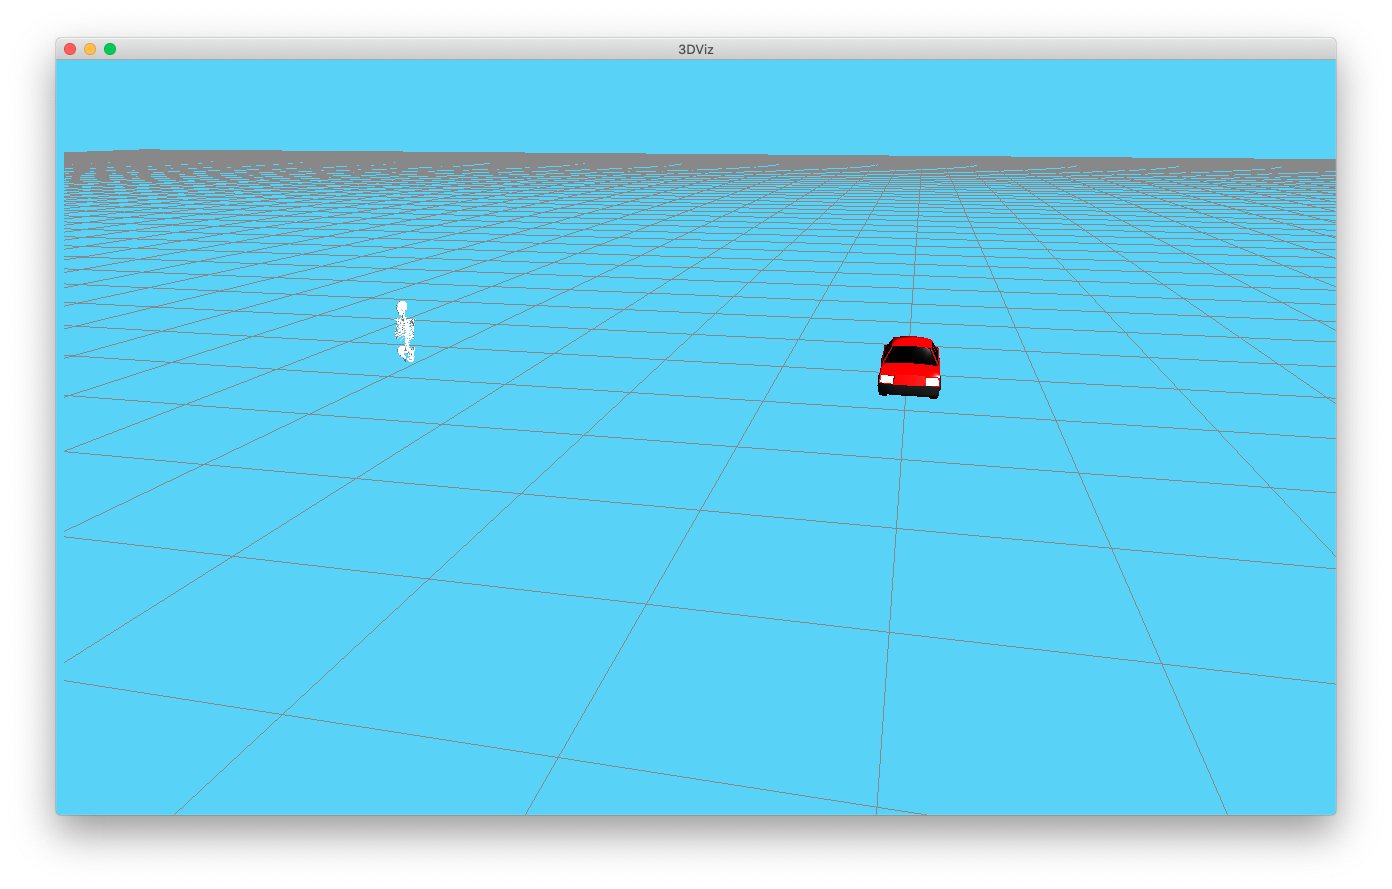
\includegraphics[width=0.8\textwidth]{figures/visualizarmodel.png}
		\caption{Dos objetos 3D mostrados en el visor}
		\label{fig.visualizarmodel}
		\end{center}
\end{figure}
\subsubsection{Movimiento de los objetos 3D}
A diferencia de un punto o un segmento, en los que es sencillo eliminarlo y volver a crearlo en la nueva posición, un objeto 3D interesa reubicarlo a la nueva posición en lugar de eliminarlo y crearlo de nuevo. Recrearlo conllevaría tener que enviar una URL o un texto plano con el archivo del objeto y cargarlo de nuevo, teniendo un retardo y carga de trabajo importante para el visor.

Al haber identificado el objeto mediante un \texttt{id} único (en el caso del punto y la recta, el \texttt{id} es el mismo para cada elemento), 3DVizWeb permite realizar el movimiento.


\begin{lstlisting}[caption= Código para realizar el movimiento de los objetos 3D, label=cod.moverobjetos]
function moveObj(objeto){
	selectedObject = scene.getObjectByName(objeto.id);
	selectedObject.position.set(objeto.x, objeto.z, objeto.y);
	selectedObject.rotation.set(objeto.rx, objeto.rz, objeto.ry);
}
\end{lstlisting}

Mover el objeto es mucho más rápido y sencillo que eliminarlo y crearlo de nuevo. Primero se selecciona el objeto mediante el identificador, posteriormente se reubica el objeto seleccionado a las nuevas coordenadas y se aplica la nueva orientación. La figura 5.7 corresponde a los objetos de la figura 5.6 desplazados y rotados:

\begin{figure}[H]
  \begin{center}
    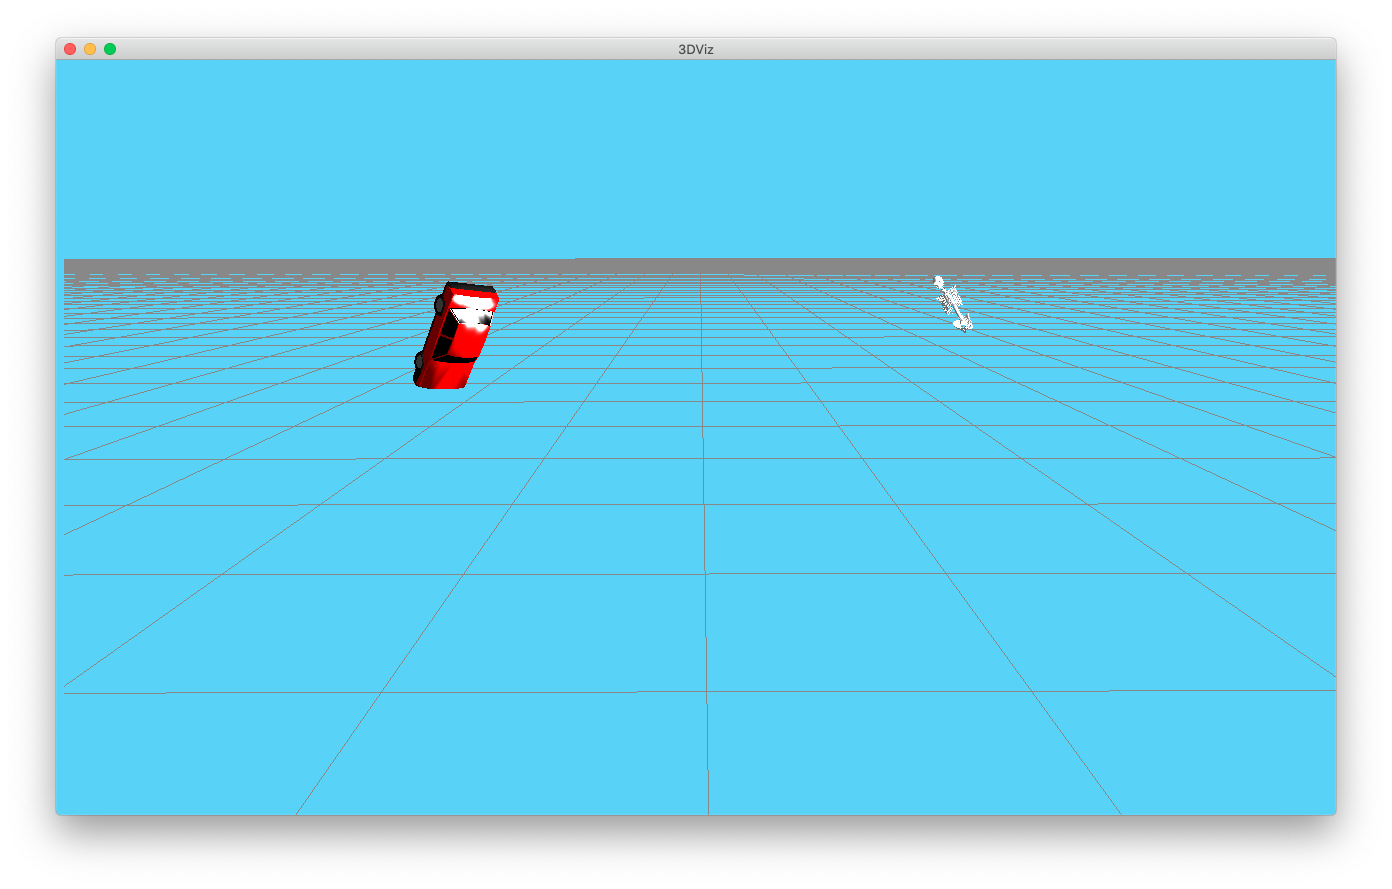
\includegraphics[width=0.8\textwidth]{figures/movermodelos.png}
		\caption{Objetos 3D reubicados y rotados}
		\label{fig.movermodelos}
		\end{center}
\end{figure}
\subsection{Borrado de elementos mostrados en el visor}
El visor ofrece dos posibilidades de borrado, la primera es borrado total de lo que se mostraba previamente en el visor, la segunda posibilidad es el borrado parcial del visor, de modo que solo se borran los elementos indicados por la aplicación.

\begin{lstlisting}[caption= Código para realizar el borrado de elementos mostrados en el visor, label=cod.borrarelementos]
function deleteObj(id){
	if (id == ""){
		delete_list = id_list;
		id_list = ["points","line"];
		id_obj = [];
	} else if (id == "obj"){
		delete_list = id_obj;
		id_list = ["points","line"];
		id_obj = [];
	} else {
		delete_list = [id];
	}
	for (i = 0; i < id_list.length; i++){
		var selectedObject = scene.getObjectByName(delete_list[i]);
		while (selectedObject != null) {
			scene.remove(selectedObject);
			selectedObject = scene.getObjectByName(delete_list[i]);
		}
	}
}
\end{lstlisting}

El código del cuadro 5.8 primero verifica cuál es el tipo de borrado, analizando la variable \texttt{id} que se pasa por parámetro. Si esta variable no tiene valor, el borrado es completo y la lista para borrar es la que contiene todos los identificadores de todos los elementos que se muestran en la escena, si toma el valor ``obj'' la lista a borrar es la correspondiente a la que contiene los identificadores de los objetos 3D. Por último, si toma el valor ``line'' o ``points'', la lista está formada únicamente por este identificador.

El borrado es selectivo por lo que para realizarlo previamente se debe haber identificado el elemento que se desea borrar y seleccionarlo en la escena mediante el identificador. Dado que la escena puede tener múltiples elementos con el mismo identificador (los segmentos y los puntos), es necesario realizar varias iteraciones buscando los elementos de la escena que el identificador coincida con el deseado hasta eliminar todos los elementos de la escena que lo tienen, ya que la llamada a \texttt{getObjectByName} solo devuelve un elemento, y no todos.

\section{Estructura de los Mensajes}
En esta sección se describe la estructura de los mensajes que intercambian la aplicación y 3DVizWeb para solicitar la visualización de cada tipo de primitiva 3D, ya sea punto, segmento u objeto. También cómo se definen utilizando el lenguaje de descripción Slice, explicado en el capítulo 3 de esta memoria. 
\subsection{Mensaje para visualizar los puntos}
Para representar un punto únicamente se necesita una posición en el eje de coordenadas y el color que tendrá el punto. Teniendo en cuenta esto, la estructura del mensaje es muy simple:
\begin{itemize}
\item Coordenada ``X''
\item Coordenada ``Y''
\item Coordenada ``Z''
\item Componente de color ``R'' (valor decimal entre 0 y 1)
\item Componente de color ``G'' (valor decimal entre 0 y 1)
\item Componente de color ``B'' (valor decimal entre 0 y 1)
\end{itemize}

Esta estructura es definida mediante el lenguaje Slice de la siguiente forma en el archivo ``primitives.ice'', que contiene las definiciones de las estructuras intermedias creadas para definir estructuras más complejas y definitivas:

\begin{lstlisting}[caption= Definición de la estrucutra del punto con Slice, label=cod.puntoslice]
#ifndef PRIMITIVES_ICE
#define PRIMITIVES_ICE

module jderobot{
	struct RGBPoint{
      		float x;
      		float y;
      		float z;
      		float r;
      		float g;
      		float b;
	};
};
#endif
\end{lstlisting}

El visor tiene la iniciativa de las comunicaciones ICE y solicitará si hay nuevos puntos que mostrar cada cierto periodo de tiempo. Dado que puede interesar que este periodo sea largo para evitar constantes peticiones y mayor carga de trabajo, se ha decidido que no solo se pueda enviar un punto en cada petición, sino que se pueda enviar un buffer de puntos. La estructura del mensaje, por tanto, no es una única posición en el eje de coordenadas y el color, sino una colección variable de estos elementos (podrá ser uno o más).

Para dar la posibilidad al servidor de indicar si desea añadir o eliminar lo que está pintado en ese momento en el visor (refrescar la escena que muestra el visor), al mensaje se le añade un parámetro. Éste toma el valor ``all'', si se desea eliminar todo lo que se muestra en ese momento y únicamente que se visualice lo que se transmite en ese mensaje. El valor ``part'', si lo que se desea es eliminar únicamente los elementos de este tipo y añadir los que se transmite en este mensaje al resto de elementos mostrados en la escena. O el valor ``nothing'', si únicamente se desea añadir lo recibido sin eliminar nada de lo que está pintado en la escena.
Por tanto el mensaje queda como sigue:
\begin{itemize}
\item Buffer de puntos con los siguientes parámetros:
	\begin{itemize}
	\item Coordenada ``X''
	\item Coordenada ``Y''
	\item Coordenada ``Z''
	\item Componente de color ``R'' (valor decimal entre 0 y 1)
	\item Componente de color ``G'' (valor decimal entre 0 y 1)
	\item Componente de color ``B'' (valor decimal entre 0 y 1)
	\end{itemize}
\item Refresco del visor
\end{itemize}

Esta estructura final del mensaje con el buffer de puntos y el refresco está definida en el archivo Slice ``visualization.ice'', utilizando las primitivas creadas en el archivo ``primitives.ice'':

\begin{lstlisting}[caption= Definición del buffer de puntos con Slice, label=cod.bufferptoslice]
#ifndef VISUALIZATION_ICE
#define VISUALIZATION_ICE

#include <primitives.ice>

module jderobot{

	sequence<RGBPoint> Points;

	struct bufferPoints{
		Points buffer;
		string refresh;
	};
};
#endif
\end{lstlisting}


\subsection{Mensaje para visualizar segmentos}
Para visualizar un segmento únicamente es necesario enviar la posición en el eje de coordenadas de dos puntos y el color con el que se desea visualizar el segmento. Por tanto, el mensaje que transporta los segmentos no es más que una ampliación del mensaje de los puntos. En el cuadro 5.11 se muestra como queda la definición del mensaje en el archivo ``primitives.ice''

\begin{lstlisting}[caption= Definición de la estructura del segmento con Slice, label=cod.segmentoslice]
structu Point{
	float x;
      	float y;
      	float z;
};

struct Segment{
	Point fromPoint;
	Point toPoint;
};


struct RGBSegment{
	Segment seg;
	float r;
	float g;
	float b;
};

\end{lstlisting}

Ahora es necesario definir el formato definitivo del mensaje, para ello se extenderá el archivo ``visualization.ice'' como se muestra en el cuadro 5.12.

\begin{lstlisting}[caption= Definición del buffer de segmentos con Slice, label=cod.buffersgmslice]
	
sequence<RGBSegment> Segments;
	
struct bufferSegments{
	Segments buffer;
	string refresh;
};
\end{lstlisting}

\subsection{Mensaje para visualizar un objeto 3D}
Mientras que para los segmentos y para los puntos únicamente se hace la petición sin añadir ningún parámetro a la misma, en el caso de las peticiones de un objeto 3D desde el visor 3D al servidor, se debe incluir el identificador que se le va a dar al objeto (en caso de que el servidor tenga uno para enviar), de modo que tanto visor como servidor pueden hacer corresponder las peticiones de movimiento o borrado con un objeto concreto mediante este identificador.

Para mostrar un objeto se necesita conocer el archivo que contiene el objeto 3D, el formato del archivo, la posición en el eje de coordenadas, la orientación del objeto y la escala del objeto. 
El archivo puede ser enviado de dos formas, la primera mediante una URL a un servidor externo o página web, la segunda enviando el fichero como texto plano. Esta segunda vía tiene el inconveniente de que no pueden ser enviados archivos de más de 1 MB de tamaño, por lo que si se quiere enviar un archivo más grande, debe realizarse mediante URL.

Se transmite también el formato del archivo, que como se ha explicado puede tomar los valores ``obj'' o ``dae'', para que el visor conozca el formato del objeto que se le está trasmitiendo.

La escala del objeto es un número decimal que indica el tamaño con el que se desea mostrar el objeto, permitiendo así mostrar varias veces el mismo objeto pero cambiando de tamaño (por ejemplo, podemos querer mostrar un brazo humano en diferentes tamaños para representar a un niño y a un adulto).

Por último, tanto para la posición como para la orientación se usará la clase ``Pose3D''. Esta clase está formada por las coordenadas ``X'', ``Y'' y ``Z'', la coordenada homogénea ``h'' y el cuaternión ``q0'', ``q1'', ``q2'' y ``q3'' para, usando las formulas matemáticas correspondientes, proporcionar la orientación del objeto.

El formato del mensaje tiene la siguiente estructura:
\begin{itemize}
	\item Archivo con el objeto 3D
	\item Formato del archivo
	\item	Pose3D
	\begin{itemize}
		\item Coordenada ``X''
		\item Coordenada ``Y''
		\item Coordenada ``Z''
		\item Coordenada homogénea``h''
		\item Cuaternión ``q0''
		\item Cuaternión ``q1''
		\item Cuaternión ``q2''
		\item Cuaternión ``q3''
	\end{itemize}
	\item Escala
	\item Identificador
	\item Refresco del visor
\end{itemize}
Como se puede ver, se vuelve a enviar el identificador que había sido previamente asignado y transmitido por el visor, y se añade también el refresco al igual que en los puntos y los segmentos. Sin embargo, debido a las limitaciones de tamaño de los archivos que se pueden enviar mediante ICE, y la necesidad de establecer un identificador común, solo es posible enviar un objeto 3D por petición realizada y no un buffer de objetos, como sí se hace con los puntos y los segmentos.

La clase ``Pose3D'' es definida en un nuevo archivo Slice llamado ``pose3d.ice'':

\begin{lstlisting}[caption= Definición de la clase Pose3D con Slice, label=cod.pose3dslice]
#ifndef POSE3D_ICE
#define POSE3D_ICE

module jderobot{

  class Pose3DData
  {
		float x;
		float y;
		float z;
  		float h;
		float q0;
		float q1;
		float q2;
		float q3;
  };

}; 
#endif
\end{lstlisting}

Este mensaje queda definido en el archivo Slice ``visualization.ice'', al tratarse de un formato final y no de una primitiva (se trata de una estructura de mensaje final y no una estructura intermedia para crear nuevas). Además, es necesario incluir al principio la referencia al archivo `pose3d.ice'':

\begin{lstlisting}[caption= Definición de la estructura del objeto 3D con Slice, label=cod.obj3dslice]
#include <pose3d.ice>
	....
  	struct object3d {
    		string obj;
    		string id;
    		string format;
    		float scale;
    		Pose3DData pos;
    		string refresh;
  	};

 \end{lstlisting}


\subsection{Mensaje para mover los objetos 3D}
Los objetos 3D que se visualizan probablemente se desee moverlos de posición u orientación,  por lo que ha sido necesario incorporar una secuencia de petición y envío de movimiento. Solo se comenzará a realizar la petición de movimiento una vez se muestre un objeto ya en el visor. La estructura de este mensaje es una versión reducida del mensaje para crear un objeto. En este caso únicamente se envía la nueva posición mediante la clase ``Pose3D'' y el identificador del objeto que se desea mover. Por tanto, la estructura queda de la siguiente manera:
\begin{itemize}
	\item	Pose3D
	\begin{itemize}
		\item Coordenada ``X''
		\item Coordenada ``Y''
		\item Coordenada ``Z''
		\item Coordenada homogénea``h''
		\item Cuaternión ``q0''
		\item Cuaternión ``q1''
		\item Cuaternión ``q2''
		\item Cuaternión ``q3''
	\end{itemize}
	\item Identificador
\end{itemize}

Este mensaje queda definido en el archivo ``visualization.ice'', al tratarse de un movimiento y no de un elemento nuevo:

\begin{lstlisting}[caption= Definición de la estructura del movimiento de los objetos 3D con Slice, label=cod.movimientoslice]
struct PoseObj3D{
	Pose3DData pos;
	string id;
 };
\end{lstlisting}

Se puede enviar una secuencia de movimientos para uno o más objetos, por lo que, al no tener el impedimento del tamaño de los archivos o del identificador, se decide permitir el envío de buffers con estas secuencias de movimiento. Si entre petición y petición se ha movido por ejemplo un objeto real varias veces, que se puedan realizar esos movimientos al mismo tiempo en el visor, evitando largos retardos que provocarían enviar los movimientos de uno en uno. En esta ocasión el campo refresco no se envía. El \textit{timing} para actualizar el movimiento está establecido en el fichero de configuración del visor.
La estructura final del mensaje es la siguiente:
\begin{itemize}
	\item Buffer de movimientos
	\begin{itemize}
		\item	Pose3D
		\begin{itemize}
			\item Coordenada ``X''
			\item Coordenada ``Y''
			\item Coordenada ``Z''
			\item Coordenada homogénea ``h''
			\item Cuaternión ``q0''
			\item Cuaternión ``q1''
			\item Cuaternión ``q2''
			\item Cuaternión ``q3''
		\end{itemize}
		\item Identificador
	\end{itemize}
\end{itemize}

El mensaje final queda definido de la siguiente forma en el archivo ``visualization.ice'':

\begin{lstlisting}[caption= Definición del buffer de movimientos con Slice, label=cod.buffermovslice]
sequence<PoseObj3D> bufferPoseObj3D;
\end{lstlisting}

\section{Conexiones}
En esta sección se describe cómo se realiza la conexión y la posterior recepción de cada uno de los objetos y objetos 3D anteriormente indicados. La conexión se realiza mediante el middleware ICE y su lenguaje de especificación Slice. Primero se detalla cómo se realiza la conexión con la aplicación que quiere usar el visor y la posterior petición de cada tipo de objeto. Finalmente se explica cómo se realiza la recepción de cada objeto y el tratamiento que recibe cada uno para su posterior visualización en el visor.

\subsection{Conexión y peticiones a la aplicación}
Para la conexión e intercambios con la aplicación, el visor hace uso de los Web Workers de HTML5\footnote{\url{https://www.w3schools.com/html/html5_webworkers.asp}} que permiten ejecutar código en segundo plano sin bloquear al proceso principal. Su uso es imprescindible para que el hilo principal no se bloquee y pueda mostrar los elementos que se reciban mientras espera la recepción del resto de peticiones realizadas. En la figura 5.8 se muestra el esquema del funcionamiento del Worker:

\begin{figure}[H]
  \begin{center}
    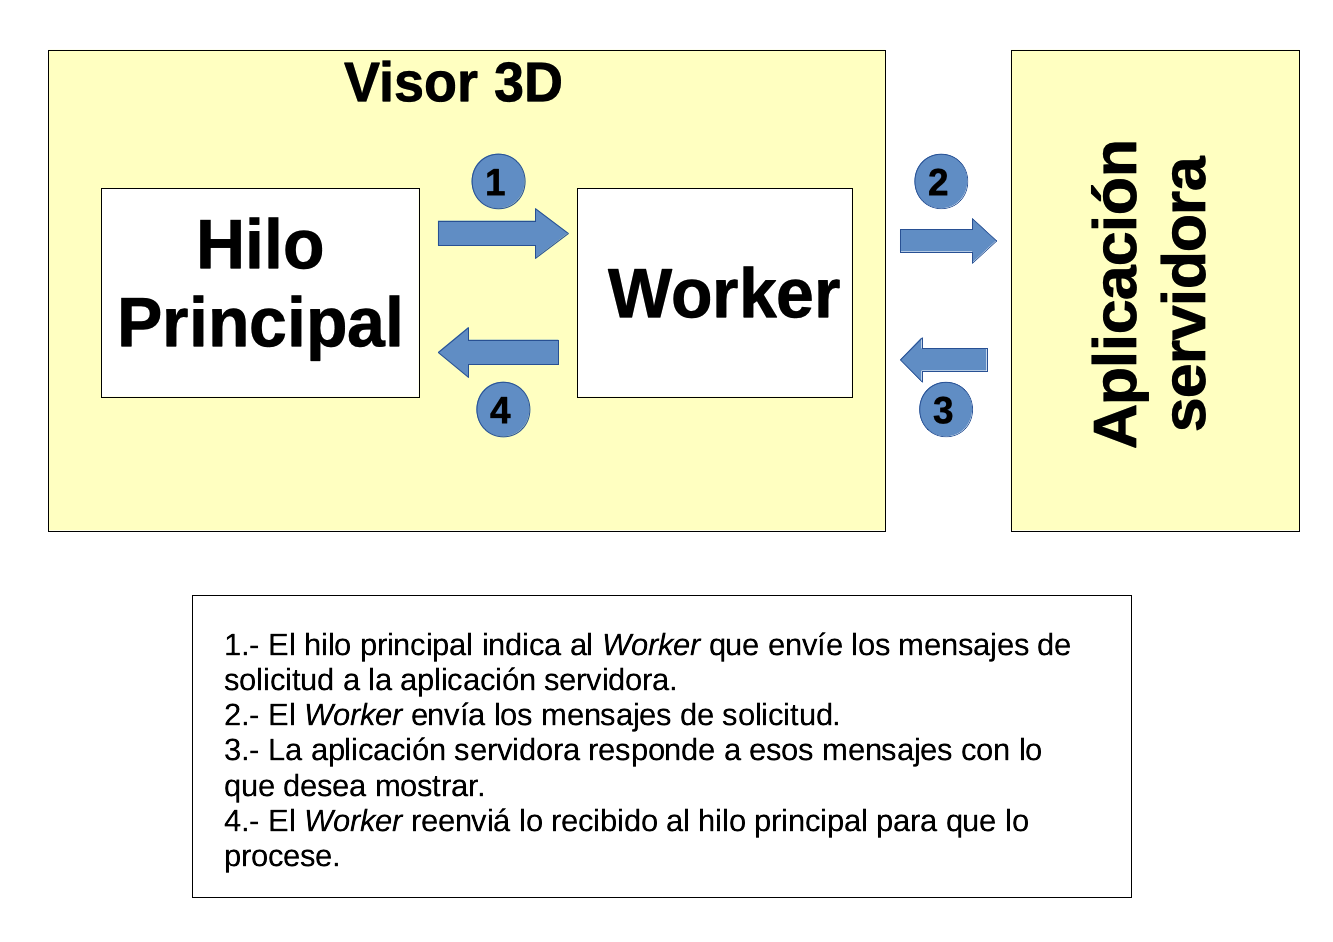
\includegraphics[width=0.8\textwidth]{figures/esquemaworker.png}
		\caption{Esquema de funcionamiento del Web Worker en el Visor 3D}
		\label{fig.diseno3dviz}
		\end{center}
\end{figure}

Una vez que el visor se ha lanzado y se ha terminado de cargar, se crea el Web Worker y se envía el mensaje para que se establezca la conexión. Esto se realiza utilizando el código del cuadro 5.16

\begin{lstlisting}[caption= Creación del Worker, label=cod.worker]
w = new Worker("js/3DViz_worker.js");
w.postMessage({func:"Start",server:config.Server, port:config.Port});
\end{lstlisting}

Cuando se ha creado el Worker se inicializa la conexión ICE que devuelve un objeto \texttt{Ice.Communicator}, que es el objeto principal para establecer una comunicación ICE. Posteriormente se crea un objeto con la interfaz indicada anteriormente para realizar la conexión. También se inicializan las variables para posteriormente lanzar el \textit{Promise} (permite manejar la naturaleza asíncrona de ICE) y la variable donde se guardará el \textit{proxy} con la conexión realizada con el servidor. Esta secuencia de código se puede visualizar en el cuadro 5.17.

\begin{lstlisting}[caption= Código para la inicialización de la conexión ICE, label=cod.inicializarice]
var ic = Ice.initialize();
var communicator;
var Promise;
var Prx = jderobot.VisualizationPrx;
var srv;
\end{lstlisting}

Una vez incializada la conexión ICE, creado el objeto con la interfaz y recibido en el \textit{Worker} el mensaje para que se establezca la conexión, se comienza el proceso para realizarla. Lo primero que se debe realizar es crear el \textit{endpoint} mediante la IP y el puerto indicado en el fichero de configuración, después se crea un \textit{proxy} realizando una petición al servidor mediante la llamada a \texttt{stringToProxy}, pasándole como parámetro una cadena de texto que contiene la identidad del objeto (será a partir de la cual el servidor sea capaz de identificar a qué \textit{proxy} se está intentando conectar el cliente) y el \textit{endpoint}. El \textit{proxy} que devuelve es del tipo \texttt{Ice.ObjectPrx}, pero realmente lo que se necesita es un \textit{proxy} a la interfaz creada en ``visualization.ice'', que se hará mediante una petición \textit{Promise}, el objeto con la interfaz y el \textit{proxy} que se acaba de recibir. Esta petición pregunta al servidor si el \textit{proxy} que ha devuelto es un \textit{proxy} para el objeto de la interfaz de ``visualization.ice''. Si lo es devuelve un \textit{proxy} del tipo \texttt{jderobot.VisualizationPrx} que se guarda en la variable creada para almacenar la conexión. Si no, devuelve un error.  Finalmente, el \textit{Worker} manda un mensaje al hilo principal indicando que la conexión se ha realizado correctamente. Todo esto se realiza mediante el método \texttt{connect} que se muestra en el cuadro 5.18

\begin{lstlisting}[caption= Código para realizar la conexión ICE, label=cod.conexionice]
function connect(server,port){
  endpoint = "ws -h " + server + " -p " + port;
  var proxy = ic.stringToProxy("3DViz:" + endpoint);
  Promise = Prx.checkedCast(proxy).then(
      function(printer)
      {
          srv = printer;
          self.postMessage({func:"Connect"});
      });
}
\end{lstlisting}

Cuando el hilo principal recibe el mensaje indicando que la conexión ha sido exitosa establece las llamadas periódicas (utilizando el tiempo indicado en el fichero de configuración) a las funciones que se encargan de realizar las peticiones al servidor mediante el método de HTML \texttt{setInterval()}\footnote{\url{https://www.w3schools.com/jsref/met_win_setinterval.asp}} como se muestra en código del cuadro 5.19. Si no lo ha sido elimina el \textit{Worker} e imprime el mensaje por consola. 

\begin{lstlisting}[caption= Código para crear las llamadas periódicas a las funciones encargadas de realizar las peticiones al servidor, label=cod.funcionesinterval]
w.onmessage = function(event) {
      	 if (event.data.func == "Connect"){
		pointInterval = setInterval(function(){
					setPoint();
						}, config.updatePoints);
		lineInterval = setInterval(function(){
					setLine();
					},config.updateSegments);
		objInterval = setInterval(function(){
					setObj();
					},config.updateModels);}	
        } else {
          console.log(event.data);
          w.terminate();
        }
\end{lstlisting}

Cuando se pase el tiempo, se activan las funciones que envían el mensaje al \textit{Worker} para que realice las peticiones al servidor. Estas peticiones serán para todos los objetos igual salvo en el caso de la petición de los objetos 3D, que como se ha explicado anteriormente, enviará el identificador que se dará al objeto en caso de que haya uno. Este identificador será una cadena de ``obj'' y un contador de objetos que hay en la escena, es decir, si no hay objetos en la escena, el siguiente tendrá de identificador ``obj1'', el siguiente ``obj2'' y así sucesivamente. Finalmente, esta función termina realizando una llamada a la función que se encarga de gestionar las respuestas del servidor. Esta secuencia de código se puede ver en el cuadro 5.20

\begin{lstlisting}[caption= Definición de las funciones de petición, label=cod.funcionespeticion]
function setPoint(){
      w.postMessage({func:"setPoint"});
      getData();
}
function setLine(){
	w.postMessage({func:"setLine"});
	getData();
}
function setObj(){
	id = "obj" + cont;
	w.postMessage({func:"setObj", id: id});
	getData();
}
\end{lstlisting}

En el \textit{Worker}, cuando se reciban los mensajes que solicitan pintar cada tipo de elemento al servidor, se realiza la petición usando el proxy con la conexión y las funciones definidas en la interfaz Slice explicada anteriormente. Si a la petición se recibe respuesta, se reenvía al hilo principal para su manejo.

\begin{lstlisting}[caption= Código que realiza las peticiones al servidor, label=cod.peticiones]
function setPoint(point){
 	srv.getPoints().then(function(data){
		self.postMessage({func:"drawPoint",points: data});
	});
}

function setLine(){
	srv.getSegment().then(function(data){
      		self.postMessage({func:"drawLine", segments: data});
  	});
}

function setObj(id){
  	srv.getObj3D(id).then(function(data){
    		self.postMessage({func:"drawObj", obj: data});
  	});
}
\end{lstlisting}

Como se puede ver en el cuadro 5.21, solo se están realizando las peticiones para los puntos, los segmentos y los objetos, pero no para los movimientos de los objetos, ya que solo se realiza una vez que se ha recibido un objeto para mostrar. Una vez que se tiene un objeto, se activa la llamada periódica a la función para que envíe el mensaje al \textit{Worker} para que se realice la petición al servidor de la misma forma que las demás.

Las funciones para realizar las peticiones al servidor se han tenido que definir previamente mediante el lenguaje de descriptivo de ICE, Slice. Para realizar la definición se ha extendido el archivo ``visualization.ice'' explicado en la sección 5.4. A este archivo se le añade la descripción del cuadro 5.22.

\begin{lstlisting}[caption= Código añadido a las definiciones Slice creadas, label=cod.extensionslice]
interface Visualization
	{
	      bufferSegments getSegment ();
	      bufferPoints getPoints();
	      object3d getObj3D(string id);
	      bufferPoseObj3D getPoseObj3DData();
	};
};

\end{lstlisting}

\subsection{Recepción y tratamiento de los mensajes recibidos}
Ya se ha explicado cómo se conecta, cómo se envían los mensajes de petición al servidor y cómo se recibe la respuesta en el Worker que la transmite al hilo principal. Ahora se explicará cómo trata esos mensajes el hilo principal para mostrarlo en el visor.

En el hilo principal hay un manejador de mensajes que es la función \texttt{getData()}, se invoca cada vez que se realiza una petición. En esta función se analiza el mensaje que se recibe procedente del \textit{Worker}. Se revisa cuál es el tipo y se realizan las tareas previas necesarias para posteriormente visualizar el elemento usando los métodos explicados en la sección 5.3. El condicional que se muestra en el cuadro 5.23 es el encargado de realizar este análisis.

\begin{lstlisting}[caption= Manejador que analiza los mensajes recibidos, label=cod.manejador]
function getData (){
	w.onmessage = function(event) {
		if (event.data.func == "drawPoint"){
			...
		} else if (event.data.func == "drawLine"){
			...
		} else if (event.data.func == "drawObj") {
			...
		} else if (event.data.func == "pose3d") {
			...
		}
	}
}
\end{lstlisting}

\subsubsection{Tratamiento de los puntos}
Si el mensaje enviado por el \textit{Worker} es del tipo \texttt{drawPoint}, el manejador indicará que se deben ejecutar las sentencias correspondientes a la visualización de los puntos. Lo primero que se realiza es verificar si el servidor ha solicitado que haya refresco del visor total, parcial o que no haya refresco, si el servidor ha indicado que se debe refrescar el visor (y si el mensaje trae puntos que mostrar, ya que si no se interpretará el mensaje como erróneo), se llama al método encargado de eliminar todos o algunos de los elementos que se muestran en ese momento en el visor y que se explica en la sección 5.3.5. 

Tanto si se ha refrescado como si no, se recorre el buffer de puntos mediante un bucle \texttt{for}, invocando al método encargado de mostrar un punto en el visor, en cada iteración hasta que ya no queden más puntos para mostrar. Al método se le pasa por parámetros el punto completo (coordenadas y componentes RGB), ya que se encarga de diferenciar cada uno y realizar las tareas necesarias para mostrarlos. En el cuadro 5.24 se muestra la secuencia de código que realiza lo descrito anteriormente.

\begin{lstlisting}[caption= Código para tratar los mensajes con los puntos, label=cod.tratarpuntos]
if (event.data.func == "drawPoint"){
	if (event.data.points.buffer.length !=0){
		if (event.data.points.refresh == "all"){
			deleteObj("");
		} else if ((event.data.points.refresh == "part")) {
			deleteObj("points");
		}
	}
	points = event.data.points.buffer;
	for (var i = 0; i < points.length; i+=1) {
        		addPoint(points[i]);
	}
}
 \end{lstlisting}

Dado que el tratamiento de los segmentos es muy similar al tratamiento de los puntos, no se profundiza en ello.

\subsubsection{Tratamiento de los objetos 3D}
El tratamiento de los objetos 3D comienza revisando si requiere refresco, o no, del visor. Una vez que se ha borrado, o no, el contenido del visor, se actualiza el contador que constituye el identificador que se ha indicado en las secciones anteriores. Posteriormente es necesario realizar la conversión de la ubicación y orientación enviada como ``Pose3D'' a un formato que el método encargado de mostrar los objetos sea capaz de entender.

Para realizar esta conversión, lo primero es crear una clase de JavaScript cuya estructura contendrá los parámetros que se necesitan para mostrar el objeto, es decir la posición en el eje de coordenadas (coordenadas ``x'', ``y'' y ``z''), las orientaciones en cada eje de coordenadas (orientación ``rx'', ``ry'' y ``rz'') y el identificador del objeto 3D. La creación de esta clase se muestra en el cuadro 5.25.

\begin{lstlisting}[caption= Definición de la clase que proporciona la posición de un objeto 3D, label=cod.clasepos]
class obj3DPose {
	constructor(id, x, y, z, rx, ry, rz){
		this.id = id;
		this.x = x;
		this.y = y;
		this.z = z;
		this.rx = rx;
		this.ry = ry;
		this.rz = rz;
	}
}
\end{lstlisting}

Para realizar la conversión se han creado tres funciones diferentes: \texttt{getYaw}, \texttt{getRoll} y \texttt{getPithc}. Estas funciones devuelven la orientación en cada uno de los ejes de coordenadas, usando las formulas matemáticas que transforman los cuaterniones en los ángulos usados para describir la orientación de un objeto tridimensional y que son un tipo de ángulos de Euler\footnote{\url{https://en.wikipedia.org/wiki/Conversion_between_quaternions_and_Euler_angles}}. Este sistema es muy utilizado en navegación de los aviones y drones, y están formados por la dirección (``yaw''), elevación (``pitch'') y ángulo de alabeo (``roll'') correspondiendo respectivamente a la orientación en el eje ``z'', el eje ``y'' y el eje ``z''.

Finalmente se crea una función que devuelve un objeto de la nueva clase creada y que tiene ya la conversión (cuadro 5.26). A esta función se le pasa por parámetro el objeto completo recibido y, mediante la llamada a las funciones para realizar la conversión, crea el objeto de la nueva clase que contendrá el identificador, las coordenadas ``x'', ``y'' y ``z'', sin ningún tipo de conversión, y las orientaciones en cada eje convertidas y que están en radianes.

\begin{lstlisting}[caption= Función que devuelve la posición tras la conversión, label=cod.posicionconvertida]
function getPose3D(data){
	var rotateZ=getYaw(data.pos.q0, data.pos.q1, data.pos.q2, data.pos.q3);
	var rotateY=getPitch(data.pos.q0, data.pos.q1, data.pos.q2, data.pos.q3);
	var rotateX=getRoll(data.pos.q0, data.pos.q1, data.pos.q2, data.pos.q3);
	var objpose3d = new obj3DPose(data.id, data.pos.x, data.pos.y,
						data.pos.z, rotateX, rotateY, rotateZ);
	return objpose3d;
}
\end{lstlisting}

Una vez que ya hemos realizado la conversión se llama al método encargado de cargar los objetos en el visor y que se explicó en la sección 5.3.4. A este método, se le pasa por parámetro el objeto completo recibido del servidor y el objeto de la nueva clase que incorpora la conversión de la orientación, para que pueda mostrar el objeto en el visor. Tras ello, se arranca la petición periódica de movimientos para el objeto (si no estaba arrancada previamente) al tener ya mínimo un objeto para mover. Esta secuencia de código se puede ver en el cuadro 5.27.

\begin{lstlisting}[caption= Código para tratar los mensajes con el objeto 3D, label=cod.tratarobjetos]
else if (event.data.func == "drawObj") {
	if (event.data.obj.obj !=""){
		if (event.data.obj.refresh == "all"){
			deleteObj("");
		} else if ((event.data.obj.refresh == "part")) {
			deleteObj("obj");
		}
	}
	cont += 1
	var pos = getPose3D(event.data.obj);
	addObj(event.data.obj,pos);
	if (posInterval == null){
		posInterval = setInterval(function(){
			setPose3D();
		}, config.updatePose3D);
	}
}	
\end{lstlisting}

\subsubsection{Tratamiento del movimiento de los objetos}
En el caso de los mensajes con el movimiento únicamente se recorrerá buffer que contiene todos los movimientos realizando la conversión de Pose3D al formato admitido e invocando al método que materializa el movimiento de los objetos. 

En la clase que se ha creado para la conversión se incluye el identificador del objeto que se va a mover, ya que, en este caso solo pasamos por parámetro la nueva clase por lo que es necesario incluir el identificador.

\begin{lstlisting}[caption= Código para tratar los mensajes con los movimientos de los objetos 3D, label=cod.tratarmovimiento]
else if (event.data.func == "pose3d") {
	for (var i = 0; i < event.data.bpose3d.length; i += 1){
		data = event.data.bpose3d[i];
		var objpose3d = getPose3D(data);
		moveObj(objpose3d);}
	}
}
\end{lstlisting}

\section{Experimentos}
El visor está preparado para ser usado principalmente con Electron, ya que la lectura del fichero de configuración solo está habilitada si se usa con Electron. Se puede utilizar en el navegador web, pero la configuración será la que se indica al visor por defecto, no pudiendo modificarse, lo que limita en gran manera las funciones del mismo. La ejecución con Electron se realiza de la misma manera que se explicó en la sección 3.8.

Para ejecutar 3DVizWeb y realizar pruebas, se ha creado una aplicación de test en python que envía un coche rotado como objeto 3D, segmentos que forman una carretera y puntos que crean una barrera limitando los bordes de la carretera .

\begin{enumerate}
\item En un terminal ejecutar el servidor de prueba:

\begin{lstlisting}[caption= Ejecutar servidor de prueba, label=cod.testserver]
#>python server_test.py
\end{lstlisting}

\item En otro terminal, ejecutar 3DVizWeb

\begin{itemize}
\item Como aplicación web utilizando Node.js\footnote{\url{https://www.youtube.com/watch?v=1fMw6iklIUs}}
\end{itemize}
\begin{lstlisting}[caption= Ejecución con Node.js, label=cod.dronenodejs]
#>node run.js
Se arranca el navegador y se introduce la URL http://localhost:7777/
\end{lstlisting}
\begin{itemize}
\item Como aplicación de escritorio con Electron\footnote{\url{https://www.youtube.com/watch?v=-lKj8eAktMI}}
\end{itemize}
\begin{lstlisting}[caption= Ejecución con Electron, label=cod.droneelectron]
#>npm install
#>npm start
\end{lstlisting}

\end{enumerate}

A continuación se muestra la prueba realizada con el servidor, tomando varias secuencias del mismo experimento:

\begin{figure}[H]
  \begin{center}
    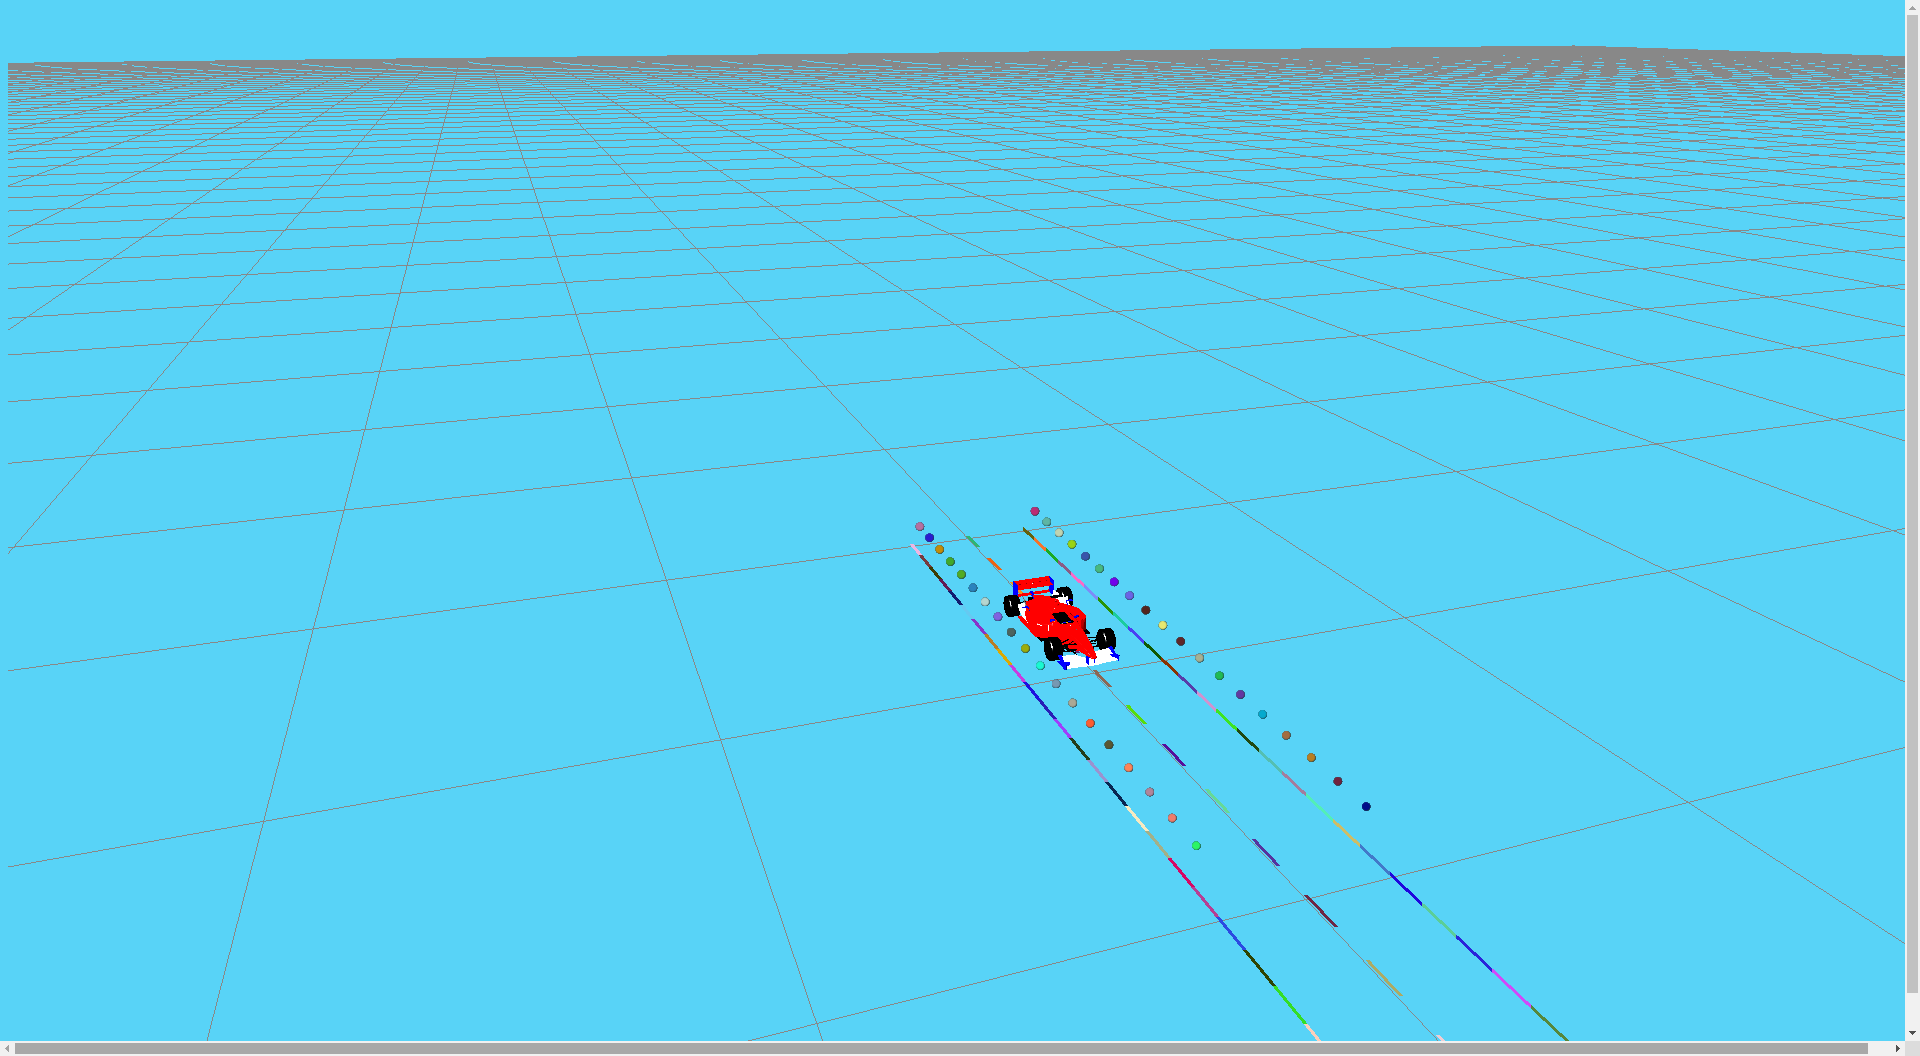
\includegraphics[width=0.8\textwidth]{figures/3DVizWeb.png}
    		\caption{Test realizado en Electron}
		\label{fig.test3dviz1}
		\end{center}
\end{figure}













